\RequirePackage[l2tabu, orthodox]{nag}

\documentclass[11pt,a4paper]{book}

\usepackage[english]{babel}
\usepackage[T1]{fontenc}
\usepackage[utf8]{inputenc}

\usepackage{microtype}
\usepackage{mathtools}
\usepackage{todonotes}
\usepackage{graphicx}
\usepackage{blindtext}
\usepackage[hidelinks]{hyperref}
\usepackage{pdfpages}
\usepackage{fullpage}

\usepackage{csquotes}
\usepackage{booktabs}
\usepackage{standalone}
\usepackage{amssymb}

\usepackage{tcolorbox}
\tcbuselibrary{listingsutf8,breakable,theorems,skins}
%The paper size for this thesis is the Swedish format s5
\usepackage{siunitx}
\usepackage{lmodern}
\usepackage{verbatim}
\usepackage{todonotes}
\usepackage{subcaption}
\usepackage{ntheorem}
\usepackage{paralist}
\usepackage[noabbrev]{cleveref}
\usepackage{braket}
\usepackage{tipa}
\usepackage{multirow}
\usepackage{textcomp}

\usepackage{caption}

\usepackage{mathptmx}
\usepackage[symbol]{footmisc}
\usepackage{makeidx}
\usepackage{helvet}
\usepackage{tikz}
\usepackage{pgfplots}
\usepackage{rotating}
\usepackage[section,acronym]{glossaries}

\graphicspath{{./graphics/}}
\definecolor{theWhite}{gray}{0.9}
\definecolor{theBlack}{gray}{0.2}

%% If the following definition throws an error, you'll need a newer version of your
% Latex distribution (from at least the second half of 2013)
\newtcbinputlisting[]{\commandline}[2][]{%
    oversize,
    colback=theBlack,
    colframe=red!50!white,
    coltext=theWhite,
    listing only,
    listing options={language={bash},aboveskip=0pt,belowskip=0pt,nolol,
    basicstyle=\ttfamily\bfseries,extendedchars=true},
    enhanced,
    breakable,
    lines before break=4,
    listing file={#2},
    arc=8pt,
    #1
}

\newcommand{\Mfig}[1]{%
\begin{figure}[<+htpb+>]
    \centering
    \missingfigure{#1}
    \caption{#1}
\end{figure}}



\begin{document}

\title{Trionic 7 Documentation}
\author{Dilemma, typeset in \LaTeX by Jonathan Jogenfors}

\maketitle
\clearpage
\listoftodos
\chapter{Introduction}
This document is intended for Saab fanatics and engineers who want to start
understanding the Saab Trionic 7 motor management system. It will give as much
information as possible about the technical part of the system. The only
limitation will be the knowledge of the author. In short the content of this
document will enable you to understand Trionic 7 better and give you hands-on
information about altering the maps it uses. Prerequisites are minor electronics
and computer knowledge and of course some understanding of how a turbo charged
engine works. Throughout the document the T7Suite software will be referenced.
This software will enable you to really “get into” the Trionic. The T7Suite
software can be downloaded from the T7Suite website.

\section{Acknowledgements}
The author would like to thank everyone on ecuproject for their help on getting
all this information together. Special thanks go out to General Failure, J.K.
Nilsson, Hook, Hma, Vigge, Mackan, Sandy Rus, JKB, L4staero and Steve Hayes.

\tableofcontents

\chapter{Hardware}
The T7 is build around a Motorola MC68332 (CPU32) microcontroller. This is a 32
bit controller that handles the entire motor management including fuel
injection, ignition timing and boost pressure control. The processor has a vast
4Mb (512 Kbyte) flash memory for fetching program code and maps. This flash
memory consisting of a AM29F400BT-90SI (AMD) holds the program memory. There is
a coprocessor from Philips, a P83C592FHA/019. This is a 8-bit 8051-based
microcontroller with a CAN (Controller Area Network) module. As the CAN physical
line driver there is an Intel AN82527 (same family as used in Trionic 5). RAM
memory is done by two 32 Kbit SRAM chips (U62H256S1K). There is also a special
component that would appear to be a barometric pressure sensor.

\section{Integrated Circuit List}
The table below lists almost all IC’s on the board. This is just to give you an idea on what to expect.

\begin{table}
    \centering
    \begin{tabular}{llll}
        Partnumber & Function & Usage & \# on board \\
        \midrule
        TC55257DFI-85L & SRAM & (working memory) & 1 \\
        16233970 & Microcontroller & Main 32-bit CPU & 1 \\
        PC83C592 & Microcontroller with CAN contr.& 8-bit coprocessor & 1 \\
        AM29F400 & Flash memory & 4 Mbit & 1 \\
        51862 & DA converter & & 1 \\
        AN82527 & CAN controller    CAN line driver & 1 \\
        16238669 0H11 & Pressure sensor? & &  1
    \end{tabular}
    \caption{}
    \label{tab:}
\end{table}

\section{Block Schematic Diagram}
\begin{figure}[<+htpb+>]
    \centering
    \missingfigure{}
    \caption{}
    \label{fig:}
\end{figure}

\section{DI Cassette}
The DI cartridge has a trigger input for firing the four individual sparkplugs. These are triggered by
signals from the ECU on pin 9, 10, 11 and 12 which are generated in the power driver IC CA3236 on
the Trionic PCB (topside, 16 pin DIL housing). Internally these four pins are connected as shown in
the table and the image below.

\begin{table}
    \centering
    \begin{tabular}{cccc}
        DI cartridge pin & ECU pinnumber &  CA3236 pinnumber &  Description \\
        \midrule
        2 & 7 & 1 (OUT A) & Trigger cylinder 1 \\
        3 & 8 & 3 (OUT B) & Trigger cylinder 2 \\
        4 & 67 & 6 (OUT C) & Trigger cylinder 3 \\
        5 & 68 & 8 (OUT D) & Trigger cylinder 4 \\
    \end{tabular}
    \caption{}
    \label{tab:}
\end{table}

\chapter{Flashing}
The Trionic 7 ECU binary images uses several checksums to verify integrity. Most
of them have been easy to figure out, but one of them is so complicated, that it
seems to been done to deter map changing. There are still some unknowns, that
would be nice to figure out. For example, I've discovered some binaries don't
seem to have all four checksums. And of course there could be more checksums
that have gone unnoticed. Two of the checksums are in the end of the binary and
the other two are scattered in the code. The latter ones can be found by using
pattern searching. Again the calculations are pretty simple, and even the harder
checksum is easy to implement. Big thanks to solving these things goes to Tomi
and General Failure.

\section{Checksum lexicon}
First of all, there are four different checksums. They have been given names by
Tomi: FB checksum, F2 checksum, Misc checksum and Area 70000 checksum.

\section{F2 and FB checksums}
The first two checksums, FB and F2, can be found at the end of the binary. This
end area has been called the file header (footer would be more logical). See
also \todo{Add reference}chapter Trionic 7 file header. The F2 checksum is not
present in all binaries, so be aware of this. Finding the two other checksums is
more of a challenge.

\section{Misc. checksum}
The Misc checksum resides inline within the code. It is usually found in the
area of 0x02000...0x05000. The checksum address can be found by pattern
searching the bin file using a set of hex values along with mask bits. If a mask
bit is not set, the corresponding hex value does not have to match. Here are the
hex values, and the masks.
Pattern
\begin{verbatim}
0x48,0xE7,0x00,0x3C,0x24,0x7C,0x00,0xF0,0x00,0x00,0x26,0x7C,0x00,0x00,0x00,0x00,0x28,0x7C,0x00,0xF0,0x00,0x00,0x2A,0x7C
\end{verbatim}
Mask
\begin{verbatim}
1, 1, 0, 0, 0, 0, 1, 1, 1, 1, 0, 0, 0, 0, 1, 1, 1, 1, 0, 0, 0, 0, 1, 1
\end{verbatim}
So, we are searching the binary for a string of bytes beginning with 0x48, 0xE7, 0x00, 0x3C... Then
we mask out the bytes that change from binary to binary. When we’ve located this pattern, we know
where to start. Now we start primitively disassembling the code. we search for byte patterns
[0x48,0x6D], [0x48,0x78], [0x48,0x79], [0x2A,0x7C] and [0xB0,0xB9]. The three first patterns reveal
addresses and lengths of checksum areas. There are 15 checksums areas from which the Misc
checksum is calculated. The [0x2A,0x7C] pattern gives a base address for the [0x48,0x6D] addresses.
Bear with me. These [0x2A,0x7C] addresses are summed with the base address to make the actual
address. This way the address is only 2 bytes long. On the [0x48,0x79] addresses it's 4 bytes long
without any base address. And the [0x48,0x78] pattern gives 2 bytes which correspond with the
length of the checksum area. Finally the [0xB0,0xB9] pattern is followed by 4 bytes to the address of
the Misc checksum.


\section{Area 70000 checksum}
This checksum refers to an area in the region of 0x70000. Like the Misc checksum, there is no clean
way of finding out the length of the area along with the checksum address. Using pattern searching
with this also has results. There are binaries that are incompatible with this approach, so this requires
some fixing in the future.
Pattern
\begin{verbatim}
0x20,0x3c,0x00,0x00,0x11,0x52,0x2F,0x00,0x20,0x3C,0x00,0x00,0x09,0xD0,0x2F,0x00,0x20,0x3C,0x00,0x00,0x00,0xCC,0xD0,0x9F
\end{verbatim}
Mask
\begin{verbatim}
1, 1, 0, 0, 0, 0, 1, 1, 1, 1, 0, 0, 0, 0, 1, 1, 1, 1, 0, 0, 0, 0, 1, 1
\end{verbatim}


After finding that pattern, the masked addresses are summed together. In the pattern, the original
addresses are 0x00001152, 0x000009D0 and 0x000000CC. Summing these gives the Area 70000
length of 0x1BEE. At the same time this is the address where to find the Area 70000 checksum.

\section{How to calculate a checksum}
The FB checksum shares the same calculation method as Misc and Area 70000 checksums. It's simply
a sum of the bytes from the checksum area. Four bytes are made into a 32 bit value and summed
with the next 32-bit value. This goes on until there are fewer than 4 bytes left. The last 1...3 bytes are
then individually summed together with the checksum.

\section{Misc checksum}
The Misc checksum is a sum of the individual checksums calculated from 15 areas. The checksum
calculation used is the same as with the FB checksum.

\section{Area 70000 checksum}
Once you have found the length of the Area 70000, you can calculate the checksum by using the
function described in section “FB checksum”. The start address is 0x70000. Notice that your binary
might not have this area present.

\chapter{Firmware}

Once you are done with dumping the flash contents and you want to do more than
only alter variables and maps you can start analyzing the binary. This is a
difficult task because there are a lot of different firmware versions, stock
ones – maybe different per MY and tuned ones that differ for every manufacturer
and stage. In every case the code can be disassembled using a 6833x disassembler
like the one in IDAPro. There are scripts available to automatically disassemble
the code and make it more readable by replacing addresses by variable names that
are extracted from the symboltable inside the binary.

\chapter{Symbol table}
Each T7 firmware file contains a symbol table describing data structures in the
program. The major problem is that from some point in time SAAB started to
compress the symbol tables in the binary file. Probably just to save space in
the flash memory but it has made tuning a little harder. We actually need these
symbol names because they tell us what a certain memory location means. For
unpacked binaries these symbols can be extracted together with their
corresponding memory addresses (ROM and RAM).


\begin{figure}[<+htpb+>]
    \centering
    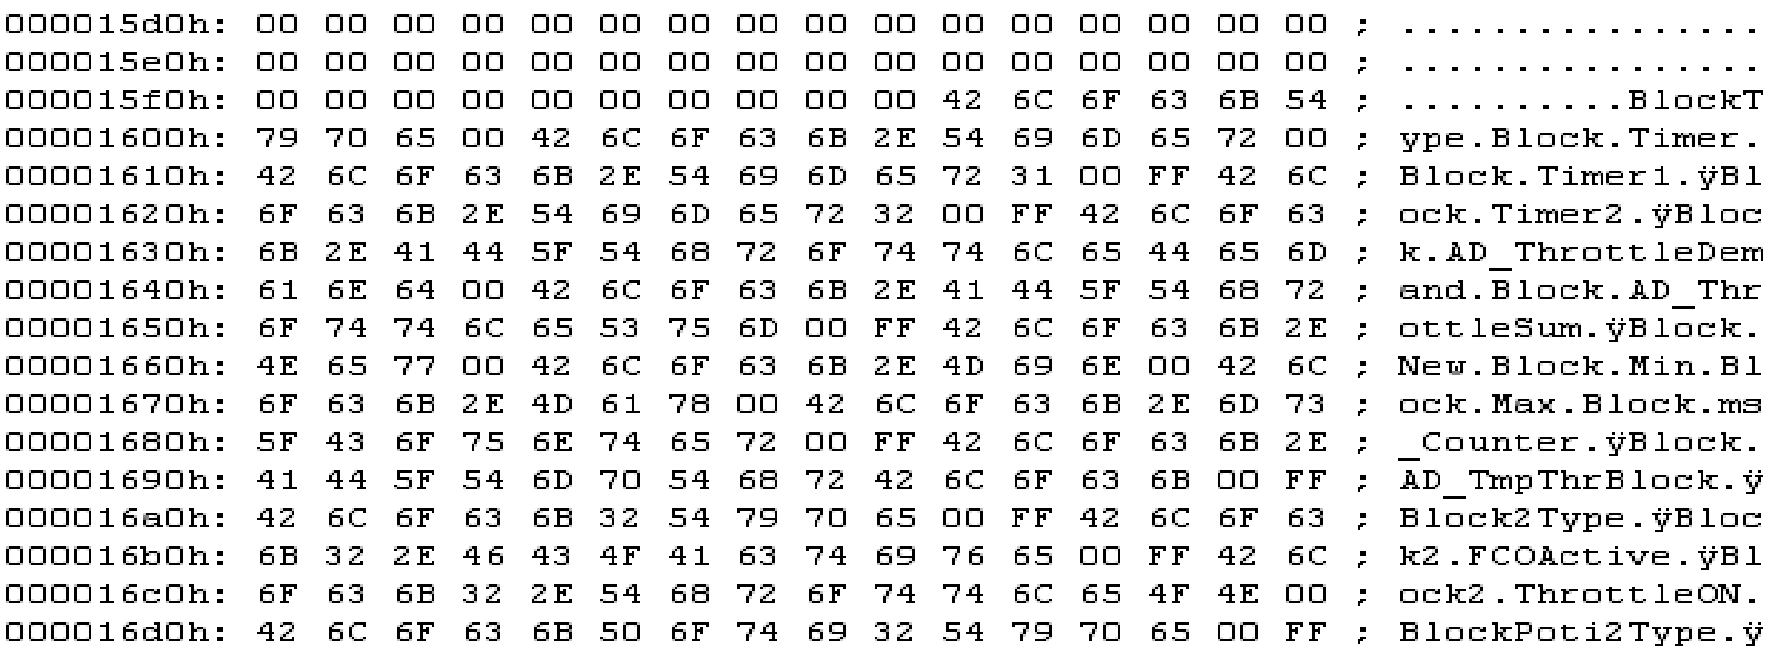
\includegraphics{symboltable.png}
    \caption{}
    \label{fig:}
\end{figure}


While examining the symbol table you can see that the separator is 0x00. In contrast to T5 where
symbol and SRAM addresses reside in the same table, we now only find the symbol name. In another
table in the binary we can find flash addresses and lengths in the same sequence as the symboltable.

\section{Finding start of symbol table:}

Search binary for string the first sequence of 15 zeros.
\section{Finding start of address lookup table:}
Search binary for 20 00 00 00 XX YY 00 F0 where XX YY is the index of the first symbol found in the
symbollist.

To save you the time to lookup all addresses manually the T7Suite application will extract all symbol
information in one run. Symbol name, flash address and length will be displayed all together.

This \todo{link}image (6) will give you an idea of what the symbol table should look like once it has been
extracted. See \todo{link}appendix I for a complete list of known symbols.
\begin{figure}[<+htpb+>]
    \centering
    \missingfigure{}
    \caption{}
    \label{fig:}
\end{figure}

When the user double clicks one of the symbols that has a flash address attached to it, T7Suite will
display the corresponding symbol in a viewer. This viewer will display the data in table form was well
as in graphical form.
\begin{figure}[<+htpb+>]
    \centering
    \missingfigure{}
    \caption{}
    \label{fig:}
\end{figure}


\chapter{Maps}
A lot of maps in the T7 are not only made up of a piece of raw data. It also
includes x-axis and y-axis information. T7Suite will automatically display all
known axis information when a map is opened. In Trionic 7 most symbols have an
English name (Trionic 5 has lots of Swedish names) that explains lots about its
function. Also, the symbols are categorized by name, which makes browsing the
symbols much easier. All torque calibration symbols start with “TorqueCal.”.
T7Suite groups all symbols by their respective category by default.

\section{Fuel}
Fuel calculation in Trionic 7 is based on the Airmass entering the engine. In rough steps this seems to
be the calculation’s flow:

\begin{description}
    \item[Basic calculation of fuel quantity per combustion] The current air mass/combustion is divided by 14.7
        and sent to box 2. The unit is now in mg
        fuel/combustion
    \item[Compensation] In case of a cold engine, shortly after starting, rapid
        load changes, knocking or high loads, the current
        value is multiplied by a compensation factor
    \item [Closed loop] The closed loop value is used as a multiplier. The
        value is then sent to box 4
    \item[Correction for purge] Multiply by the value for purge adaptation. The
        value is sent to box 5
    \item[Multiplicative adaptation (long term fuel trim)] The multiplicative adaptation value is used as a
        multiplier and the new value is sent to box 6
    \item[Additive adaptation] The additive adaptation value is added and the new
        value is sent to box 7
    \item[Starting fuel quantity] If the engine has not yet started, starting fuel is
        selected. The value is sent to box 8
    \item[Fuel quantity per combustion to be injected] The fuel quantity per combustion is the amount of
        petrol to be supplied to the engine. The value is sent
        to box 9
    \item[Injector opening duration] Converts the value to the time during which the
        injector must be open and the new value is sent to
        box 10
    \item[Injection twice per combustion] Injection takes place twice per combustion until the
        camshaft position has been found. Injection duration
        is divided by two. The value is sent to box 11
    \item[Voltage dependant needle lift duration added
        (battery correction)]
        Adds the injector time delay, which is voltage
        dependant. The value is sent to box 12
    \item[ Fuel cut] The value is sent to box 13 unless fuel cut is active
    \item[ Activation of injector] At a DETERMINED crank shaft angle, the
        microprocessor will control the transistor for the
        injector that is next in the firing order
\end{description}
The basic fuel quantity is calculated based on Airmass and Injector constant. This injector constant is
called InjCorrCal.InjectorConstant.
\begin{figure}[<+htpb+>]
    \centering
    \missingfigure{}
    \caption{}
    \label{fig:}
\end{figure}
If the engine is not warmed up yet, an alternate fuel map is used called BFuelCal.StartMap. If the
engine has reached operating temperature the normal map “BfuelCal.Map” is used.
\begin{figure}[<+htpb+>]
    \centering
    \missingfigure{}
    \caption{}
    \label{fig:}
\end{figure}


You will see the areas calibrated to be run in closed loop have a value of around 1.00. It can be .98-
1.02 or so. Then you will notice the high load part of the maps ramp up to enrich the mixture.
The trick is to set the closed loop part of the map first, the areas that are represented by values of
1.00.

You will need to switch closed loop off and drive around with a wideband in the tailpipe.
What you want to achieve is an AFR of 14.7 for petrol while driving around under light loads where
the value is 1.00. What T7 does is calculate the injection time to be say 5ms, if that is not correct it is
multiplied by this map. Say you need to enter a value of 1.1 in the map to get correct AFR it will
change injection time to 5.5ms (5ms*1.1=5.5ms)

The idea is to get closed loop area correct first. This will stop any negative adaption once the tune is
finished and allowed to run in closed loop again. If the closed loop area of your fuel map is too rich it
will negatively adapt over a long period of time. This will have the effect of leaning your AFR's across
the board.

Example: you make a tune, closed loop AFR's are fine (because the O2 is making it fine through
feedback) but unknown to you its rich and short term fuel trim is driving negatively 13%. I.e. is
leaning off injection time by 13\%.

You don’t notice this and make some full power runs to check AFR its fine at say 12.5 AFR.
After several weeks the multiplicative adaptation (Long term fuel trim) has absorbed some adaption
and has earned a value of -13\% this will now subtract 13\% from whole fuel calculation including full
power. All of a sudden your full power AFR has jumped up to 14.0 AFR, \emph{engine failure happens
very easily from here}.

Now back to fuel mapping. To set closed loop area of fuel map, monitor the AFR in this light load area
and if its wrong after adjusting for large injectors, start by just adjusting the Injector constant up and
down accordingly instead of altering the closed loop area of the BfuelCalMap. This will affect the
whole map instead of one point. By doing it this way you can almost get AFR spot on in closed loop
area just by a few goes at adjusting the injector constant.

It can be found in InjCorrCal.InjectorConst, the value represents the injectors flow in mg of fuel (not
capacity or cc's as injectors are normally rated in). The injector constant is a calculation factor used by
T7 to calculate injection time.

Once closed loop area is done the high load area can be mapped. If its too lean just increase the
values in the relative column relating to what site of the map you are running in. Once your high load
areas are done, activate closed loop again so you can see how it all runs. Monitor fuel adaptations and
AFR etc.

One thing to note is how quickly it drops into open loop under full throttle.
By going into open loop the o2 sensor is "masked" where the ECU listens to what its saying but
ignores it, this allows afr's to go beyond 14.7 and injection correction is directly taken from the fuel
map we just adjusted allowing much enrichment to cool charge etc.

To alter open loop enrichment you can change at what Airmass flow T7 switches to open loop in
LambdaCal.MaxLoadNormTab. Also, open loop entry (so, leaving closed loop situation) has a delay
attached to it. This way, short overruns of the maximum load will not immediately result in leaving
closed loop. Stock bins often have this set to 2000 milliseconds which seems quite long. If you want
to ECU to leave closed loop faster after overrunning the load limit, just decrease the time in
LambdaCal.TimeOpenLoop.
\begin{figure}[<+htpb+>]
    \centering
    \missingfigure{}
    \caption{Battery correction values for injector latency}
    \label{fig:}
\end{figure}

\begin{figure}[<+htpb+>]
    \centering
    \missingfigure{}
    \caption{Water temperature correction}
    \label{fig:}
\end{figure}


\begin{figure}[<+htpb+>]
    \centering
    \missingfigure{}
    \caption{Fuel injection correction map for knock conditions}
    \label{fig:}
\end{figure}

\begin{enumerate}
    \item Idling speed ignition timing With idle speed control active, the timing is adjusted
        to stabilize idle engine speed. The value is sent to
        box 3
    \item Normal ignition timing When idle speed control is inactive, the ignition
        timing is read from a load and engine speed
        depending matrix. The value from the matrix is
        optimized for lowest fuel consumption (best engine
        torque) and sent to box 3
    \item Selection of ignition timing One of the ignition timing calculation is selected
        depending on which function is active. The value is
        sent to box 6
    \item Catalytic converter heating timing In order to heat up the catalytic converter as fast as
        possible after start, the ignition will be retarded.
        This is a compensation matrix that is added to the
        value in box 3. The matrix is dependent on load and
        engine speed
    \item Engagement of catalytic converter heating timing The function is active when coolant temperature is
        above -10 degrees Celsius and below +64 degrees
        Celsius
    \item Total The value from box 5 is added to the value of box 3
    \item Compensation The ignition timing is corrected depending on engine
        coolant temperature and intake air temperature. The
        value is sent to box 6.
    \item Knock control If knocking occurs, a timing retardation will be
        calculated. The value is sent to box 6
    \item Total The compensation angle and knock retardation are
        totalled to give the current ignition timing. The value
        is sent to box 7
    \item Selection of ignition timing Starting ignition timing is selected when the engine
        has not been started. The value is sent to box 9
    \item Starting ignition timing Starting ignition timing is selected when the engine
        has not yet been started. The value is sent to box 9
    \item Activate relevant trigger At the calculated crankshaft angle, the
        microprocessor controls the transistor for the trigger
        that is next in firing order
\end{enumerate}
\begin{figure}[<+htpb+>]
    \centering
    \missingfigure{}
    \caption{ignition chart}
    \label{fig:}
\end{figure}

\subsection{DI Cassette}
The ignition cassette is mounted on the valve cover on top of the spark plugs. The ignition cassette
houses four ignition coils/transformers whose secondary coil is directly connected to the spark plugs.
The ignition cassette is electrically supplied with battery voltage from the main relay (B+) and is
grounded in an earth point. When the main relay is activated the battery voltage is transformed to
400 V DC which is stored in a capacitor. The 400 V voltage is connected to one of the poles of the
primary coil in the four spark coils. Connected to the ignition cassette there are four triggering lines
(from the Trionic ECU, pin 9 (cyl. 1), pin 10 (cyl. 2), pin 11 (cyl. 3) and pin 12 (cyl. 4)). When the ECU
is grounding pin 9, the primary coil for the first cylinder is grounded (via the ignition cassettes B+
intake) and 400 V is transformed up to a maximum of 40 kV in the secondary coil for cyl. 1. The same
procedure is used for controlling the ignition on the rest of the cylinders.
\Mfig{DI Cassette}

\subsection{Idle control}
\Mfig{idlecontrol}
\Mfig{Ignition is normally controlled by the main ignition matrix:
IgnNormCal.Map}

\section{Torque}
Trionic 7 is a torque/Airmass request system instead of a boost request system like Trionic 5 is.
The basic procedure for the Airmass controller is like in the table below.
\begin{enumerate}
    \item  Driver request The control module reads pedal potentiometer 1 and converts the
voltage to Airmass per combustion (mg/c). The value is sent to box 3
\item Cruise control request When cruise control is active, the air mass per combustion required to
maintain the set speed is calculated. The value is sent to box 3
\item Select highest value The control module selects the highest of the two values (box 1 or box
2). The value is sent to box 5
\item Engine torque limitation The maximum permissible air mass per combustion varies depending
on the engine type. During operation, the maximum permissible mg/c
must also be limited to protect the engine, gearbox, brakes and turbo
\item Select lowest value The control module selects the lowest value and sends it to box 8
\item Compensation request When the AC compressor is on, and when the heated rear window or
radiator fan is on, the mg/c required to compensate for the increased
load is calculated. The value is sent to box 8
\item Other air request The control module calculates the mg/c required for idle speed control.
The value is sent to box 8
\item Totalling values The control module totals all the values. The total is sent to box 9
\item Total requested mg/c
\item Total Airmass request
\item Throttle control The requested mg/c is converted to requested voltage for throttle
position sensor 1. The charge air pressure and intake air temp are
used to correct this conversion. The throttle motor rotates the throttle
until the current voltage for throttle position sensor 1 corresponds with
the requested voltage
\item Current mg/c The requested mg/c is also compared with the current mg/c (MAF
reading). If needed the requested voltage for throttle position sensor 1
is finely adjusted
\item Turbo control If mg/c is too high for throttle alone the turbo control will take over.
The excess is converted to a PWM which controls the charge air
control valve. The absolute pressure sensor is used to correct the
conversion
\item Current mg/c The requested mg/c is compared to current mg/c and the charge air
control vale PWM is finely adjusted if required
\end{enumerate}


\subsection{Torque request}
So, if the driver (or cruise control for that matter) pressed the accelerator pedal he actually requests a
certain Airmass from the system. This value is fetched from the PedelMapCal.m\_RequestMap shown
below.
\Mfig{PedelMapCal.m\_RequestMap}

The table holds Airmass values for each position of the accelerator pedal and each rpm site. Trionic
now looks up the estimated engine output (torque) based on Airmass and rpm. This is done through
map \enquote{TorqueCal.M\_NominalMap} as shown next.

\Mfig{TorqueCal.M\_NominalMap}

\section{Second lambda sensor}
In the years Trionic 7 was shipped on cars, several things changed in these cars setups. One of the
major changes was the introduction of the second lambda (oxygen, O2) sensor that is placed after the
catalyst to ensure the catalyst is working properly. If you want to run software from a double lambda
sensor car in a single lambda car, you have to make some changes in the settings. This information is
courtesy of L4staero.

\subsection{Turning off second lambda sensor}
You can use this procedure in cars having only one lambda sensor and in cars having two lambda
sensors, but with a missing catalyst.

\begin{table}
    \centering
    \begin{tabular}{lll}
Map & Value& Description \\
\midrule
LambdaCal.ST\_AdapEnable & 0 &Second lambda sensor disabled \\
LambdaCal.ST\_AdapEnable & 1& Second lambda sensor enabled \\
    \end{tabular}
    \caption{}
    \label{tab:}
\end{table}

\subsection{Alternative solution to turning off second lambda}
Change low limit on O2heaterPostCal.I\_LowLim to 0 mA to disable sensor heater error, and change
CatDiagCal.LoadHi and LoadLo to values never seen normally, like 30 and 20.

\begin{table}
    \centering
    \begin{tabular}{lll}
Map & Value & Description \\
\midrule
O2HeatPostCal.I\_LowLim& 0& \multirow{3}{*}{Second lambda sensor disabled} \\
CatDiagCal.LoadLo &20 &\\
CatDiagCal.LoadHi &30&\\
O2HeatPostCal.I\_LowLim & 230 & \multirow{3}{*}{Second lambda sensor enabled}\\
CatDiagCal.LoadLo &140 &\\
CatDiagCal.LoadHi &425 &\\
    \end{tabular}
    \caption{}
    \label{tab:}
\end{table}

\section{Calibration of OBD2 and LEV EVAP systems}
If we want to run a file that was developed for OBD2 or a LEV car in an earlier car we run into
problems because the early car is missing a second catalyst, a tank pressure sensor and a purge
canister behind the fuel tank. If you have an early B205E/L engine you simply couldn’t run a later
B205R software version in it because it would through CEL’s for the missing hardware. We need to
make changes to the file before we can run in on an earlier car (e.g. switch of the control of the new
hardware).

OBDCal.OBD2Enabled= This is self explanatory, if car is OBD2 put value at 1 if it's not OBD2 put value
at 0.

On this point in later bins(compressed) there is EOBDEnable which is always on in EC2000 EU files
and LOBDEnable which is always on in EC2000 RW files. File type is shown in firmware information
under engine type.

OBDCal.EnableOBD2Limit= As above but its a 4 byte value. If done in Hex value for a OBD2 car is
00000001 and for non-OBD2 car is 00000000. As shown in T7suite is 2 values. OBD2 cars top value is
1 and bottom value is 0. In non OBD2 car both values are 0.

OBDCal.evapEquipmentExist= If car is equipped with a canister at rear of tank and a tank pressure
sensor value will be 1. If neither exist value should be set to 0.
\subsection{Info on LEV (Low Emission Vehicle)}
For example take a 2001 9-3 Aero (or SE as called in USA) equipped with a B205R, Saab's decision to
take all "R" engines and clean them so to speak by developing new emission systems for them leaves
them with some differences to their low level engine relatives. The term LEV(Low emission vehicle) in
this sense refers to Saab's decision to add a second catalytic converter and a tank pressure sensor
and a large purge canister behind fuel tank, as well as adding a 2nd oxy to monitor condition of first
cat.

\section{Footer information}
If we look at the footer in the binary (last page in hex viewer) we see a set of reversed strings. Each
of these strings contains an identifier. These identifiers have a hardcoded meaning.

\begin{table}
    \centering
    \begin{tabular}{lll}
Identifier & Length & Description \\
\midrule
0x91& 0x09& Ecuid.vehicleidnr \\
0x94 & 0x07 & Ecuid.ecuhardwversnr \\
0x95 & 0x0C & Ecuid.ecusoftwnr \\
0x97 & 0x1E & Ecuid.ecusoftwversnr \\
0x9A & 0x04 & Ecuid.softwaredate \\
0x9C & 0x04 & variable name table crc (not really sure) \\
0x9B & 0x04 & Symboltable (packed table with symbol names) \\
0xF2 & 0x04 & F2 checksum \\
0xFB & 0x04 & Romchecksum.piareachecksum \\
0xFC & 0x04 & Romchecksum.BottomOffFlash \\
0xFD & 0x04 & RomChecksumType \\
0xFE & 0x04 & Romchecksum.TopOffFlash \\
0xFA & 0x05 & Lastmodifiedby \\
0x92 & 0x0F & Ecuid.partnralphacode (IMMO) \\
0x93 & 0x07 & Ecuid.ecuhardwnr \\
0xF8 & 0x02 & ? \\
0xF7 & 0x02 & ? \\
0xF6 & 0x02 & ? \\
0xF5 & 0x02 & ? \\
0x90 & 0x11 & Ecuid.scaletable (VIN) \\
0x99 & 0x06 & Ecuid.testerserialnr \\
0x98 & 0x0D & Ecuid.enginetype \\
0xF9 & 0x01 & Romchecksum.Error
\end{tabular}
    \caption{}
    \label{tab:}
\end{table}
\Mfig{footer}

\chapter{Tuning with T7}
\section{Tuning with T7Suite}
To get the ECU to produce more engine output, several parameters (maps) have to altered. This
chapter will give you a general idea on what to change – and why – for getting to an approximate
stage II equivalent. The example is a 9-3 B205R.

\subsection{AirCtrlCal.m\_MaxAirTab}
Airmass value from controller where area map has reached max-area and there is no point to increase
the I-part. Resolution is 1 mg/c
\Mfig{AirCtrlCal.m\_MaxAirTab}

\subsection{AirCtrlCal.m\_MaxAirE85Ta}
( if running on E85 )
Same as above for E85

\subsection{BoostCal.I\_LimTab}
Load limit tab. to enable the I Part of boost regulator. If the load request from Airmass master is
above this value plus the hysteresis is the I Part enabled and the throttle closed loop is disabled. If
the load request from Airmass master is below this value is the I Part disabled and the throttle is
allowed to run in closed loop.

\subsection{BoostCal.P\_LimTab}
Load limit tab. to enable the P Part of boost regulator. If the load request from Airmass master is
above this value plus the hysteresis is the P Part enabled. If the load request from Airmass master is
below this value is the P Part disabled.

\subsection{BoostCal.RegMap}
Main constant matrix. Resolution is 0.1 \%.

\subsection{BstKnkCal.MaxAirmass}
(divide by 3,1 for approx torque, ignition, airtemp etc affect this!)
Map for max allowed Airmass for manual gearbox, m\_nHigh. Resolution is 1 mg/c.

\subsection{BstKnkCal.MaxAirmassAu}
Map for max allowed Airmass for automatic gearbox, m\_nHigh. Resolution is 1 mg/c.

\subsection{FCutCal.m\_AirInletLimit}
If the "MAF.m\_AirInletFuel" is higher than this limit during m\_AirInletTime will the fuelcut be activated
( pressure guard ).

\subsection{IgnE85Cal.fi\_AbsMap}
( if you want to change the ignition )
Ignition map for E85 fuel. Resolution is 0.1 degrees.

\subsection{IgnNormCal.Map}
( if you want to change the ignition )
Normal ignition map. Resolution is 0.1 degrees.

\subsection{MapChkCal.CheckSum}
(automatically updated in between every map
change with T7suite!)

\subsection{MaxVehicCal.v\_MaxSpeed}
Speed limiter.

\subsection{PedalMapCal.m\_RequestMap}
Requested Airmass from the driver as a function of rpm and accelerator pedal position. Resolution is 1
mg/c.
\subsection{TorqueCal.M\_ManGearLim}
Maximum engine torque limit for each gear in the manual gearbox. Resolution is 1 Nm.

\subsection{TorqueCal.m\_AirTorqMap}
(This is where all torque limiters take their data from and therefore
needs to be "fooled" if you are running 400nm+ or an automatic!)
Data-matrix for nominal Airmass. Engine speed and torque are used as support points. The value in
the matrix + friction Airmass (idle Airmass) will create the pointed torque at the pointed engine speed.
Resolution is 1 mg/c. axis to the above map: TorqueCal.m\_AirXSP

\subsection{TorqueCal.M\_EngMaxTab}
Data-table for maximum engine out put torque for manual cars. Resolution is 1 Nm.

TorqueCal.M\_EngMaxAutTab
Data-table for maximum engine output torque for automatic cars. Resolution is 1 Nm.

TorqueCal.M\_5GearLimTab
Data-table for maximum engine output torque for manual cars on fifth gear. Resolution is 1 Nm.


TorqueCal.M\_EngMaxE85Tab ( if running on E85 )
Data-table for maximum engine output torque when running on E85. Resolution is 1 Nm.

TorqueCal.m\_PedYSP
Air mass support points for (Calc) X\_AccPedalMap. Resolution is 1 mg/combustion.

\section{Tuning Boost calibration}
This map holds percentages (0.1\% accurate) of how much air should be passed to the return hose of
the boost control value. The higher the value, to more air is bled off and the less the wastegate will
open (and thus, the more air the turbo will be spooling). As you can see, the more Airmass is
requested (x – axis) the more the wastegate is held shut and thus, the more Airmass the turbo will be
providing. If we want more Airmass from the turbo, we need to keep the wastegate shut longer and
thus we have to enter higher numbers on the right side of the table.

\section{Altering Airmass limiter}
To be able to flow more air though the engine that is allowed in the stock configuration we will have
to modify the Airmass limiter tables as well. Note that there are two different ones, one for manual
gearbox and one for automatic gearbox. This example will only show the manual gearbox table
(BstKnkCal.MaxAirmass) but for automatic cars BstKnkCal.MaxAirMassAu needs to be changes.

\Mfig{Altering airmass p37}

As you can see, the maximum amount of Airmass allowed is approximately 970 mg/c. We need to
change the table so that it will allow more Airmass. In this case we just up the
table with 25\% with
the math functions in T7Suite.
NOTE: Please do not simply turn off this limiter by setting it way higher than the actually intended
level because it is an important limiter to provide engine safety.

\section{Altering fuelcut}
Then there’s the fuelcut function to worry about. We need to increase the limit of what the fuel cut
function will accept to prevent it from shutting of fuel too early.
NOTE: Please do not simply turn off this limiter by setting it way higher as the actually intended level
because it is an important limiter to provide engine safety.


\section{Engine speed limiter}
To prevent the system to reduce Airmass above engine speeds that are still acceptable we need to
change MaxSpdCal.n\_EngLimAir as well. Y axis values are engine temperature (coolant). Please note
that 200 rpm above this limit, the fuel cut mechanism will become active!
\section{Vehicle speed limiter}
An option is to increase the vehicle speed limiter as well. In this stock binary the vehicle speed is
limited to 240 km/h. We can change it to – for example 280 km/h.


\section{Airmass request}
To get more from the engine than in the stock configuration we need to actually request more
Airmass for a certain pedal position and rpm site. This can be done through
PedalMapCal.m\_RequestMap. Because we want more power at wide open throttle (from the drivers
perspective) we need to increase the Airmass request at pedal positions in the high percentage range
(top of the table).

As you can see we increased the top two rows so that a maximum of 1350 mg/c will be requested.
In addition we need to alter the y axis support point for the pedal map that lets Trionic lookup a pedal
position for a given Airmass. This map is called TorqueCal.m\_PedYSP. This axis map should support
the maximum Airmass we’re requesting in the m\_Requestmap, so in our case we need to modify the
map to match the 1350 mg/c we are requesting as a maximum.

The map that uses this axis is called TorqueCal.x\_AccPedalMap. It it shown below with the altered
axis values for clarification.

\section{Torque limiter}
To prevent to system to reduce Airmass above a certain engine output, the torque limiter needs to be
increased according to expected engine output.

\Mfig{Torque limiters}

TorqueCal.m\_AirTorqMap (This is where all torque limiters take their data from and therefore
needs to be \enquote{fooled} if you are running 400nm+ or an automatic!)
Data-matrix for nominal Airmass. Engine speed and torque are used as support points. The value in
the matrix + friction Airmass (idle Airmass) will create the pointed torque at the pointed engine speed.
Resolution is 1 mg/c.

Finally, we’re all done!

\chapter{Automatic transmission specifics}
In automatic Trionic 7 cars the TCM (Traction Control Module) sends a torque limit over can to the
ECU (Trionic). This means – theoretically - you cannot achieve more torque than the torque limit the
TCM dictates. The only known way around this at present time is to make Trionic THINK it’s not
making that much torque, so we have to fool the ECU into thinking it is still below the torque limit set
by the TCM.

There are different TCM limits depending on year, engine type, gearbox etc.
A MY01-AERO AUT has a 330NM limiter while a 5 speed automatic gearbox has a 350Nm limit.
To fool the ECU into thinking it is making less torque is to rescale the x-axis for
TorqueCal.mAirTorqMap which is TorqueCal.M\_EngXSP. The top value in this list must be no
more than the TCM limit.

In this case the top three rows have been altered to keep the calculated torque below 330Nm.

\begin{table}
    \centering
    \begin{tabular}{ccc}
        400 & -> & 330Nm\\
        350 &-> &320Nm\\
        320 &->& 310Nm
    \end{tabular}
    \caption{}
    \label{tab:}
\end{table}
\Mfig{TorqueCal}

This means that when requesting 330Nm you will actually get 400, 320 will get you 350 and so on.
The torque limiters in TorqueCal.M\_EngMaxAutTab must be scaled with this in mind...
In this case 400Nm between 2780 and 3920rpm. Values in between you need to recalculate, at
4300rpm the user wanted 390Nm, (400=330, 350=320) means that 322=360, 324=370, 326=380,
328=390nm

\Mfig{}

If you want to use the same bin in manual cars all manual limiters must be calculated and set
correctly!

\textbf{NOTE: In Bio power bins TorqueCal.M\_EngMaxE85Tab !}

\chapter{Using the tuning wizard}
\todo{Emphasize the limitations of tuning wizard}T7Suite incorporates a tuning wizard. This wizard allows you to automatically alter the maps in the
binary file to get it to a stage I equivalent file. The wizard can be activated by selecting “Tuning” >
“Easy tune to stage I” from the menu. A dialog will appear in which you can confirm that you want to
tune the file to stage I. Once you’ve selected this the process will start. After a few seconds a report
will appear showing all actions taken on your file.

\Mfig{Tuning wizard images}

\chapter{OpenSID values}
T7Suite incorporates a function to allow visualization of information on the SID (System Information
Display). This way you can view real-time information without utilizing the Canbus interface. You can
select the variables you want the SID to display using the SID information selection option in T7Suite.

Also, the software should be opened to be able to view the selected data on the SID. This is done in
the firmware information screen.
\Mfig{OpenSID}

Some tips on how to use the SID information option:
\begin{itemize}
    \item
ECMStat.ST\_ActiveAirDem shows the current Airmass limiter
    \item
ECMStat.P\_Engine shows calculated engine power (hp)
    \item
ECMStat.AirFuelRatio shows calculated AFR
    \item
ECMStat.p\_Diff shows boost pressure (manifold – ambient) in 0.1 kPa units
    \item
BstKnkProt.MapPointer shows the offset in 0.1 degrees for BstKnk.MaxAirmass (so, the
ignition offset for knock)
    \item
ExhaustCal.ST\_Enable allows you to enable and disable the EGT algorithm. These algorithms
are based on the stock engine and won’t be properly calibrated for a stage 3+ setup.
    \item
KnkDetAdap.KnkCntCyl first 2 bytes show cylinder 1 knock count, next 2 bytes shows cylinder
2 knock count etc.
\end{itemize}

\end{document}
